\documentclass[a4paper]{exam}

\usepackage{amsmath,amssymb, amsthm}
\usepackage{geometry}
\usepackage{graphicx}
\usepackage{hyperref}
\usepackage{titling}
\usepackage{forest}

\usepackage{mdframed}

\usepackage{xcolor}






% Header and footer.
\pagestyle{headandfoot}
\runningheadrule
\runningfootrule
\runningheader{CS/MATH 113, SPRING 2025}{WC 05: Proofs}{\theauthor}
\runningfooter{}{Page \thepage\ of \numpages}{}
\firstpageheader{}{}{}

% \printanswers %Uncomment this line

\title{Weekly Challenge 05: Proofs}
\author{Blingblong} % <=== replace with your name student ID, e.g. Blingblong (xy012345)
\date{CS/MATH 113 Discrete Mathematics\\Habib University\\Spring 2025}

\qformat{{\large\bf \thequestion. \thequestiontitle}\hfill}
\boxedpoints

\begin{document}
\maketitle


\begin{questions}
    \titledquestion{Tiles from Ohio}
    Consider the the WuShrek board below (on left), and the SonicChika tiles next to it (below to the right). A SonicChika tile would cover two squares of a WuShrek board. Imagine you have an arbitrarily large supply of SonicChika tiles
    Given a WuShrek board give a formal prove/disprove for the following problems:

    \begin{center}
        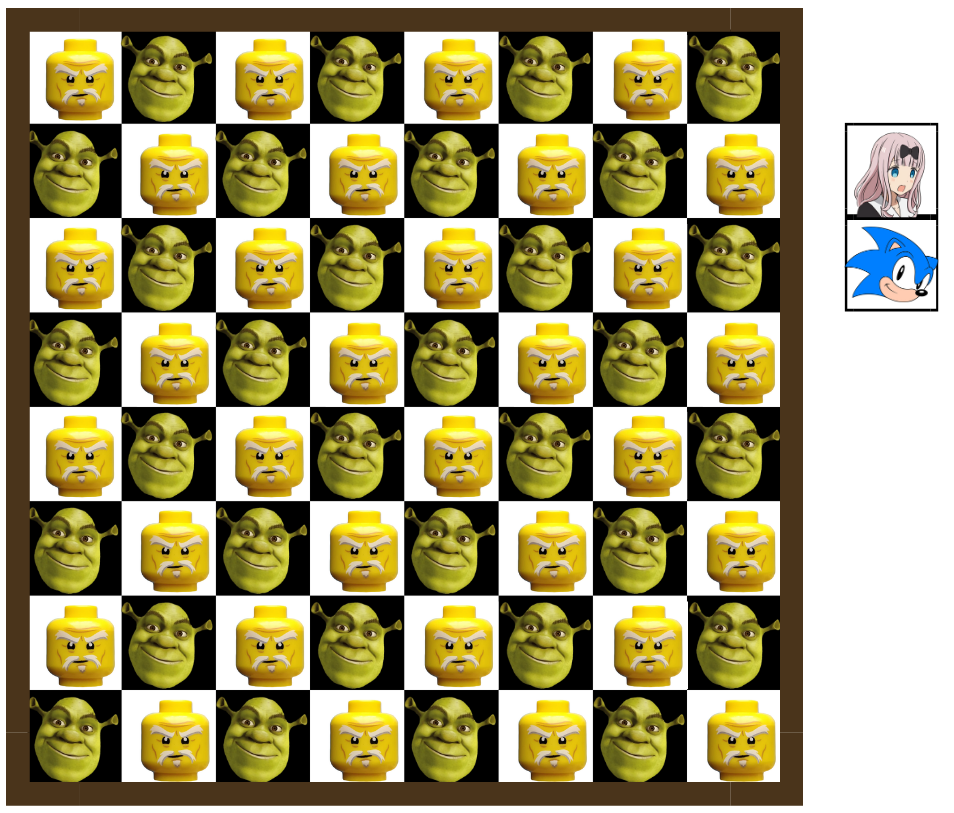
\includegraphics[scale = 0.5]{WuShrekSonicChika.png}
    \end{center}

    \begin{parts}
        \part Can you cover all the squares of the WuShrek board by using SonicChika tiles?
        \part Suppose we remove the top left square of the WuShrek board. Can you still over all the remaining squares of the WuShrek using the SonicChika tiles?
        \part Suppose we remove the top left and the bottom left squares of the WuShrek board. Can you still over all the remaining squares of the WuShrek using the SonicChika tiles?
        \part Suppose we remove the top left and the bottom right squares of the WuShrek board. Can you still over all the remaining squares of the WuShrek using the SonicChika tiles?
        \part If we remove a square with Shrek on it and a square with Wu on it from the WuShrek board (they can be any squares not necessarily adjacent), can you still cover all the remaining squares of the WuShrek using the SonicChika tiles?
    \end{parts}
    In all of the problems above no two SonicChika tiles can ever overlap.
      
\end{questions}
\end{document}

%%% Local Variables:
%%% mode: latex
%%% TeX-master: t
%%% End:
